% !TeX encoding = utf-8
% !TeX program = lualatex
% !TeX spellcheck = en_US
% !BIB program = biber
\documentclass[%singlesided,
               doublesided,
               paper=a4,
               fontsize=10pt
              ]{my-resume}

\usepackage[english]{babel}
\usepackage[
    % sorting=nyt,      % nyt | nty | nyt | nyvt | anyt | ynt | ydnt | none | debug
    % style=authoryear, % numeric | alphabetic | authoryear | authortitle | verbose | draft | debug
    % uniquename=false, % true, false , init, full, allinit, allfull, mininit, minfull
]{biblatex}
\addbibresource{Literature.bib}
\usepackage{csquotes}

%%%%%%%%%%%%%%%%%%%%%%%%%%%%%%%%%%%%%%%%%%%%%%%%%%%%%%%%%%%%%%%%%%%%%%%%%%%%%%%%
% set geometry
%%%%%%%%%%%%%%%%%%%%%%%%%%%%%%%%%%%%%%%%%%%%%%%%%%%%%%%%%%%%%%%%%%%%%%%%%%%%%%%%

\setlength\highlightwidth{8cm}
\setlength\headerheight{3.0cm}            % note that margintop gets added to this value, i.e. the header bar is 5cm
\setlength\marginleft{1cm}
\setlength\marginright{\marginleft}      % needs to be 1.5 times to be actually equal. why?
\setlength\margintop{1cm}
\setlength\marginbottom{1cm}


%%%%%%%%%%%%%%%%%%%%%%%%%%%%%%%%%%%%%%%%%%%%%%%%%%%%%%%%%%%%%%%%%%%%%%%%%%%%%%%%
% FONTS
%%%%%%%%%%%%%%%%%%%%%%%%%%%%%%%%%%%%%%%%%%%%%%%%%%%%%%%%%%%%%%%%%%%%%%%%%%%%%%%%

\RequirePackage{fontspec}
\setmainfont{Carlito}


%%%%%%%%%%%%%%%%%%%%%%%%%%%%%%%%%%%%%%%%%%%%%%%%%%%%%%%%%%%%%%%%%%%%%%%%%%%%%%%%
% COLORS
%%%%%%%%%%%%%%%%%%%%%%%%%%%%%%%%%%%%%%%%%%%%%%%%%%%%%%%%%%%%%%%%%%%%%%%%%%%%%%%%

\colorlet{highlightbarcolor}{lightgray}
\colorlet{headerbarcolor}{darkgray}

\colorlet{headerfontcolor}{white}
\colorlet{accent}{awesome-red}
\colorlet{heading}{black}
\colorlet{emphasis}{black}
\colorlet{body}{black}


%%%%%%%%%%%%%%%%%%%%%%%%%%%%%%%%%%%%%%%%%%%%%%%%%%%%%%%%%%%%%%%%%%%%%%%%%%%%%%%%
% set document
%%%%%%%%%%%%%%%%%%%%%%%%%%%%%%%%%%%%%%%%%%%%%%%%%%%%%%%%%%%%%%%%%%%%%%%%%%%%%%%%


\begin{document}

\name{Dr. Benedikt Kleinmeier}
\tagline{Computer scientist / Passion for good software / Interested in hardware and physics}
\photo[round]{Figures/Portrait/bk}{\dimexpr \headerheight-\marginbottom}   % make photo exactly match the header with margintop/marginright/marginbottom as margin

\makeheader

\highlightbar{

    \section{Contact}
    
    \begin{infolist}
        \email{kleinmeier.benedikt@gmail.com}
        % \phone{}
        % \location{}
        \homepage{Projects}{https://schwefelsaeure.github.io/portfolio/}
        \github{Github}{https://github.com/Schwefelsaeure/}
        % \linkedin{Name Surname}{https://www.linkedin.com/in/name-surname/}
        \orcid{Publications}{https://orcid.org/0000-0003-2344-8265}
        % \ads{}{}
    \end{infolist}
        
    \section{Skills}
    
    \skillsection{Programming languages}
    \skill{Assembler (x86, TriCore)}{2}
    \skill{Bash}{4}
    \skill{C}{5}
    \skill{C++}{3}
    \skill{C\#}{3}
    \skill{Java}{5}
    \skill{JavaScript}{2}
    \skill{Python}{5}
    \vspace{0.5em}
    
    \skillsection{Markup languages}
    \skill{HTML/CSS}{4}
    \skill{LaTeX}{4}
    \vspace{0.5em}
    
    \skillsection{Operating systems}
    \skill{Linux}{5}
    \skill{MacOS}{1}
    \skill{Windows}{4}
    \vspace{0.5em}
    
    \skillsection{Software and tools}
    \skill{Visualization}{3}
    (e.g. matplotlib, gnuplot, ...)\\
    \skill{Data handling/analysis}{3}
    (e.g. numpy, pandas, ...)\\
    \skill{Docker}{2}
    \skill{Office}{4}
    \vspace{0.5em}
    
    \skillsection{Process models}
    ISO26262, Scrum, V model
    \vspace{0.5em}
    
    \skillsection{Development techniques}
    Continuous integration, test-driven development
    \vspace{0.5em}
    
    \skillsection{Languages}
    \skill{German}{5}
    \skill{English}{3}

      \section{Awards}

    \cvachievement{\faTrophy}{2019}{TUM Graduate School Internationalization Grant}
    \cvachievement{\faTrophy}{2010}{Nomination scholarship program I.C.S.}
    \cvachievement{\faTrophy}{2004}{Best graduate junior high school}
}
\mainbar{
    
    \section[\faGears]{Work experience}
    \job{since 07/2021}
    {Infineon Technologies AG, Neubiberg}
    {Principal software engineer for in-house and customer tools }
    {\begin{itemize}
    		\item SDK and GUI development (PyQt) of radar applications to configure radar sensors, acquire and visualize data.
            \item Improving an Eclipse-based application to operate lab equipment and to manage cryptographic keys.
            \item Development of a Python-based workflow engine including a web dashboard to automatically process customer orders.
            \item Development of a GUI application (Swing) to control SPICE simulators and to examine simulation results.
            \item[] \tag{C++} \tag{Java} \tag{Python} \tag{GUI} \tag{PyQt} \tag{Eclipse/SWT} \tag{plotly/dash}
    \end{itemize}}

    \job{12/2017 -- 05/2021}
        {Hochschule München / Technical University Munich / University of Sussex, Munich / Brighton}
        {PhD}
        {\begin{itemize}
            \item Modeling and simulation of pedestrians and their behavioral changes.
            \item Implementation and simulation in our own open-source simulator Vadere (\url{www.vadere.org}).
            \item GUI programming in Java and data analysis using Python with a focus on test-driven development and continuous integration.
            \item[] \tag{Java} \tag{Python} \tag{JUnit} \tag{pandas} \tag{matplotlib} \tag{GUI}
        \end{itemize}}
    
    \job{05/2015 -- 11/2017}
        {Infineon Technologies AG, Neubiberg}
        {Expert firmware developer}
        {\begin{itemize}
            \item Development of bootstrap loaders and startup code for various microcontrollers in C.
            \item Establishing systematic unit testing to meet ISO 26262 requirements.
            \item[] \tag{C} \tag{Python} \tag{Ceedling}
        \end{itemize}}
    
    \section[\faMortarBoard]{Studies}
    \job{10/2012 -- 01/2015}
        {Hochschule München, Munich}
        {Computer science (M.Sc) --- embedded systems focus}
        {\begin{itemize}
            \item Master thesis at Fraunhofer ESK: Development of a software solution for highly accurate time and position detection for Car2X scenarios
            \item Focus: Driver development under GNU/Linux in C
            \item[] \tag{C} \tag{C++}
        \end{itemize}}
    
    \job{10/2008 -- 09/2012}
        {Hochschule München, Munich}
        {Computer science (B.Sc)}
        {\begin{itemize}
            \item Bachelor thesis at Infineon Technologies AG: Development of an evaluation tool for barometric air pressure sensors
            \item Focus: Firmware development for 8- and 16-bit microcontrollers in C and PC software in C\#/.NET
            \item[] \tag{C} \tag{C\#} \tag{.NET}
        \end{itemize}}

}
\makebody
\clearpage


\pagestyle{highlightmain}
\highlightbar{

    \section{Hobbies}
    \smallskip % additional skip because tag outlines use up space
    % Use \par to group two tags on one line to force a ragged-right layout.
    \tag[black]{Freestyle football}
    \tag[black]{Football}
    \par
    \tag[black]{GNU/Linux}
    \tag[black]{Mnemotechnics}
    \par
    \tag[black]{Playing the piano}
    \tag[black]{Music}
    \par
    \tag[black]{Mountainbiking}
    \tag[black]{Hiking}
    
    \section{My philosophy}
    \begin{itemize}[itemsep=1mm]
    \item Joy of learning: That's why I have been learning to play the piano autodidactically.
    \item[] 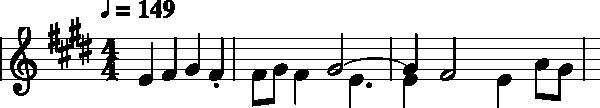
\includegraphics[width=6cm]{Figures/Interests/PianoSheet-59Improvisation-FirstLineCropped}
    \item Work-life balance and nature: For this reason, I have crossed the alps with my mountain bike.
    \item[] 
\includegraphics[width=6cm]{Figures/Interests/CirclesFilledWithNaturePictures}
    \end{itemize}

}
\mainbar{
    
    \section[\faMortarBoard]{Activities before studies}
    \job{03/2008 -- 09/2008}
    {SEP AG (backup software), Weyarn}
    {Support staff}
    {\begin{itemize}
            \item Setting up test environments (Windows, GNU/Linux), software testing, maintaining user documentation.
            \item[] \tag{GNU/Linux} \tag{Windows} \tag{Documentation}
    \end{itemize}}

    \job{03/2007 -- 11/2007}
    {Caritas St.-Anna-Haus, Holzkirchen}
    {Community service worker in retirement home}
    {\begin{itemize}
            \item Nursing and housekeeping
    \end{itemize}}

    \section[\faMortarBoard]{School}
    \job{2004 -- 2006}
        {Technical secondary school and vocational secondary school, Bad Tölz}
        {Focus: Economy and management}
        {\begin{itemize}
        		\item[] Two internships: local bank (departments: human resources, accounting, credit) and district office Miesbach
       	\end{itemize}}
    \job{2000 -- 2004}
        {Junior high school, Miesbach}
        {}
        {}
    \job{1994 -- 2000}
        {Elementary school, Weyarn}
        {}
        {}

    \section[\faFileTextO]{Publications}
    Peer-Reviewed journal articles:
    \begin{itemize}
        \item \fullcite{kleinmeier-2020}
        \item \fullcite{kleinmeier-2019}
    \end{itemize}

    \vspace{1.5em}

    \today\\[0.25em]
    
\includegraphics[width=3.5cm]{Figures/Unterschrift/Unterschrift-Kleinmeier-Vectorized}\\[0.25em]
    \textbf{Benedikt Kleinmeier}

}
\makebody

\end{document}
